\newpage
\section{Questão 12-23}

\begin{figure}[H]
	\centering
	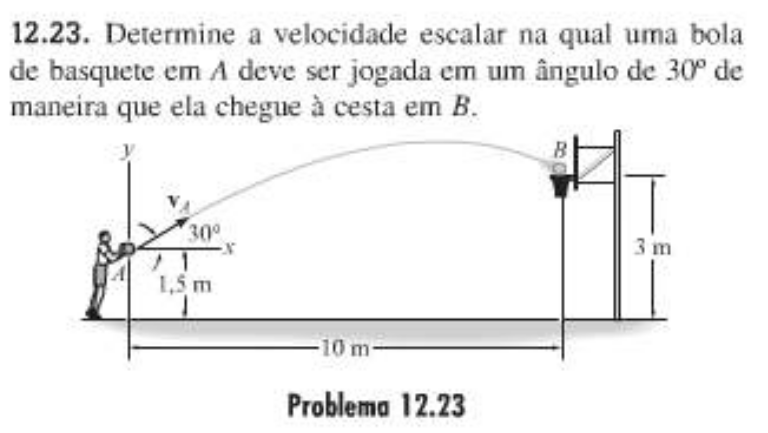
\includegraphics[width=.7\linewidth]{fundamentais/12-23.png}
	\caption{Comando da questão 12-23.}\label{fig:12-23}
\end{figure}

Nesta questão, analisamos o movimento de um projétil lançado de uma altura inicial \(y_0 = 1.5 \, \text{m}\) com um ângulo de lançamento de \(30^\circ\). O projétil percorre uma distância horizontal de \(x = 10 \, \text{m}\) e atinge uma altura final de \(y_f = 3 \, \text{m}\). Nosso objetivo é determinar a velocidade inicial \(v_A\) necessária para satisfazer essas condições.

\subsection*{Equações do Movimento}
As equações do movimento horizontal e vertical são:
\[
x = v_A \cdot \cos(\theta) \cdot t,
\]
\[
y_f = y_0 + v_A \cdot \sin(\theta) \cdot t - \frac{1}{2} g \cdot t^2,
\]
onde:
\begin{itemize}
    \item \(x = 10 \, \text{m}\): Distância horizontal;
    \item \(y_0 = 1.5 \, \text{m}\): Altura inicial;
    \item \(y_f = 3 \, \text{m}\): Altura final;
    \item \(g = 9.81 \, \text{m/s}^2\): Aceleração gravitacional;
    \item \(\theta = 30^\circ = \frac{\pi}{6}\): Ângulo de lançamento.
\end{itemize}

\subsection*{Movimento Horizontal}
Do movimento horizontal, temos:
\[
x = v_A \cdot \cos(\theta) \cdot t.
\]

Resolvendo para o tempo \(t\):
\[
t = \frac{x}{v_A \cdot \cos(\theta)}.
\]

\subsection*{Movimento Vertical}
Substituímos \(t = \frac{x}{v_A \cdot \cos(\theta)}\) na equação do movimento vertical:
\[
y_f = y_0 + v_A \cdot \sin(\theta) \cdot \frac{x}{v_A \cdot \cos(\theta)} - \frac{1}{2} g \cdot \left(\frac{x}{v_A \cdot \cos(\theta)}\right)^2.
\]

Simplificando:
\[
y_f = y_0 + x \cdot \tan(\theta) - \frac{g \cdot x^2}{2 \cdot v_A^2 \cdot \cos^2(\theta)}.
\]

Substituímos \(y_0 = 1.5 \, \text{m}\), \(y_f = 3 \, \text{m}\), \(x = 10 \, \text{m}\), \(g = 9.81 \, \text{m/s}^2\), e \(\cos(30^\circ) = \sqrt{3}/2\), \(\tan(30^\circ) = 1/\sqrt{3}\):
\[
3 = 1.5 + 10 \cdot \frac{1}{\sqrt{3}} - \frac{9.81 \cdot 10^2}{2 \cdot v_A^2 \cdot \left(\frac{\sqrt{3}}{2}\right)^2}.
\]

Simplificando:
\[
3 = 1.5 + \frac{10}{\sqrt{3}} - \frac{9.81 \cdot 100}{v_A^2 \cdot \frac{3}{4}}.
\]

\[
3 = 1.5 + \frac{10}{\sqrt{3}} - \frac{1308}{v_A^2}.
\]

\subsection*{Resolução para \(v_A\)}
Reorganizamos a equação para resolver \(v_A\):
\[
v_A^2 = \frac{1308}{3 - 1.5 - \frac{10}{\sqrt{3}}}.
\]

Calculando:
\[
v_A \approx 12.37 \, \text{m/s}.
\]

\subsection*{Resultado Final}
A velocidade inicial necessária para que o projétil atinja a altura final \(y_f = 3 \, \text{m}\) após percorrer \(x = 10 \, \text{m}\) é:
\[
v_A \approx 12.37 \, \text{m/s}.
\]
